%!TEX encoding = UTF-8 Unicode

\section{Introduction}
\label{sec:intro}

TODO shorten

% paragraph about HRC, understanding others, communication for cooperation
\IEEEPARstart{C}{ooperation} is a tenet of human society~\cite{turner:1975}, whereby humans have the ability of working successfully in groups.
This skill is acquired around the second year of life: children are able to coordinate their behavior with that of an adult partner or peer in cooperative problem-solving activities and social games, not only by mere behavioral coordination, but also by
%showing knowledge about how the different roles are interrelated, as well as
employing communicative strategies~\cite{melis:2010:rstb}.
In adulthood, understanding one another is a fundamental pre-requisite for success.
Team members typically agree on common goals~(e.g., through verbal and non-verbal communication), they work towards the execution of these goals in a coordinated way, and they understand each other's physical actions~(e.g., body movements) towards the realization of the final target.
Human team coordination and mutual understanding is effective~\cite{ramnani:2004:natureneuro} because of~(i) the capacity to adapt to unforeseen events in the environment, and re-plan one's actions in real time if necessary, and~(ii) a common motor repertoire and action model, which permits us to understand a partner's physical actions and manifested intentions as if they were our own.
% GLU
%Robotics is progressing fast, with a steady and systematic shift from the industrial domain to domestic, public and leisure environments~\cite[ch.~65, Domestic Robotics]{siciliano:2016:handbook2}. Application areas that are particularly relevant and being researched by the scientific community include: robots for people's health and active aging, mobility, advanced manufacturing~(Industry~4.0). In short, all domains that require direct and effective \hri{} and communication (including language and gestures~\cite{matuszek:2014:aaai}).
%However, robots have not reached the level of performance that would enable them to work with humans in routine activities in a flexible and adaptive way, for example in the presence of sensor noise, or unexpected events not previously seen during the training or learning phase. One of the reasons to explain this performance gap between \hh{} teamwork and a \hr{} teamwork is in the collaboration aspect, i.e., whether the members of a team understand one another. Humans have the ability of working successfully in groups. They can agree on common goals~(e.g., through verbal and non-verbal communication), work towards the execution of these goals in a coordinated way, and understand each other's physical actions~(e.g., body gestures) towards the realization of the final target. Human team coordination and mutual understanding is effective~\cite{ramnani:2004:natureneuro} because of~(i) the capacity to \emph{adapt} to unforeseen events in the environment, and re-plan one's actions in real time if necessary, and~(ii) a common motor repertoire and action model, which permits us to understand a partner's physical actions and manifested intentions as if they were our own~\cite{saponaro:2013:crhri}.

% paragraph about social sobots, need for learning/adaptation of language
Even though social robots\footnote{A social robots is ``[a robot that is] able to communicate and interact with us, understand and even relate to us, in a personal way. [It] should be able to understand us and itself in social terms''~\cite{breazeal:2002:dsr}.} are becoming ever more present in domestic, public and leisure environments~(thanks to the rapid technical advancements that touch all aspects of robotics: sensors, actuators, and algorithms), the performance of \hh{} teams is still superior to that of \hr{} teams.
Putting socially intelligent machines alongside common human users~(as opposed to specialized factory technicians as has been done in industrial robotics since the 1960s), bears issues and challenges.
For instance, the communication skills possessed by a robot cannot be entirely pre-programmed, because we cannot possibly model all the possible verbal and non-verbal~(e.g., gestures) cues that can take place during \hri, due to the richness of language and the high variability of the real world outside of laboratories and factories.
For this reason it is necessary to have robots that \emph{learn} elements and properties of language and communication, and the ability to link these elements with other skills, such as other perceptual modalities~(e.g., vision of objects of the world, vision of other agents' physical actions) and manipulation abilities~(e.g., grasping objects and moving them in order to achieve a goal)~\cite{steels:2003:trendscogsci}.

% paragraph about developmental robotics
One way to endow robots with adaptability and learning in the real world is the growing field of developmental robotics~\cite{lungarella:2003:devrobsurvey,cangelosi:2015:devrobbook}.
It takes inspiration from the progressive learning phenomena observed in children's mental development~(e.g., the understanding of language, the acquisition of manipulation skills, the understanding of others' actions), and investigates how to model the evolution and the learning of these increasingly complex cognitive processes.
In this line of research, robots are experimental platforms, being used to verify theoretical models of emergence and development of cognition.
The rationale is the following: if a model is instantiated inside a system physically embedded in the real world, many things can be learned about its strengths and limitations.
%This is often achieved with probabilistic and statistical methods. TODO ADD REF

% paragraph about neuroscience, and correspondence problem in robotics
In neuroscience research, visuomotor neurons~(i.e., neurons that are activated by visual stimuli) have been a subject of ample study~\cite{rizzolatti:2001:nrn}.
Mirror neurons are one class of such neurons that responds to action and object interaction, both when the agent acts and when it observes the same action performed by others, hence the name ``mirror''.
We show that, using this theory, a robot can first acquire knowledge by sensing and self-exploring its surrounding environment~(e.g., by interacting with available objects and building up an affordance representation of the interactions and their outcomes) and, as a result, the robot is capable of generalizing its acquired knowledge while observing another agent~(e.g., a human person) who performs similar physical actions to the ones executed during prior robot training.
This tackles the so-called correspondence problem~\cite{nehaniv:2002:correspondence} in our simple collaboration scenario, assuming that the two agents have a similar body~(i.e., a humanoid robot and a human) and operate on a shared space~(i.e., a table accessible by both agents' arms).

% paragraph summarizing our contributions and comparing with the GLU article
This article is an extention of our recent work~\cite{saponaro:2017:glu}.
We combine robot ego-centric learning about language and object affordances~\cite{salvi:2012:smcb} with the observation of external agents by gesture recognition~\cite{saponaro:2013:crhri}.
Our novel contributions are:
(i)~a probabilistic method to fuse self-learned knowledge of language and object affordances, with socially aware information of others' physical actions~(in the form of uncertain soft evidence);
(ii)~experimental findings showing the reasoning power of our combined system, which is able to make inferences and predictions over affordances and words% by incorporating the estimation of external agents
; and
(iii)~the possibility of generating verbal descriptions from the estimated word probabilities, with emergence of non-trivial language properties such as congruent/incongruent conjunctions, subjects being repeated between two consecutive sentences speaking about the same concepts.

Furthermore, we make our human action data and probabilistic reasoning code publicly available\footnote{\url{https://github.com/gsaponaro/tcds-gestures} - this page access will be made available at publication time.} in the interest of reproducibility.

The article is structured as follows. TODO ToC

%GLU
% This work takes inspiration from the theory of mirror neurons, and contributes towards using it on humanoid and cognitive robots. We show that a robot can first acquire knowledge by sensing and self-exploring its surrounding environment~(e.g., by interacting with available objects and building up an affordance representation of the interactions and their outcomes) and, as a result, the robot is capable of generalizing its acquired knowledge while observing another agent~(e.g., a human person) who performs similar physical actions to the ones executed during prior robot training. Fig.~\ref{fig:experimental_setup} shows the experimental setup.

%PHOTOS FROM OCTOBER 2017, NOT USED
% Below are the human-robot images from the external view (camera on a tripod)
% TODO: if we don't use them, purge seq2-*.png from the repo history
% \begin{figure*}
%     \centering
%     \subfloat
%     { 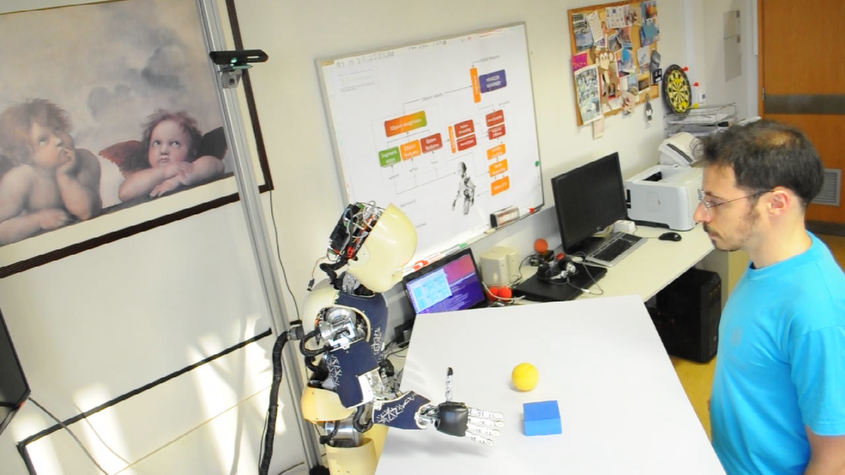
\includegraphics[width=\myWidth\linewidth]{seq2-grasp-11} } \quad
%     %
%     \subfloat
%     { 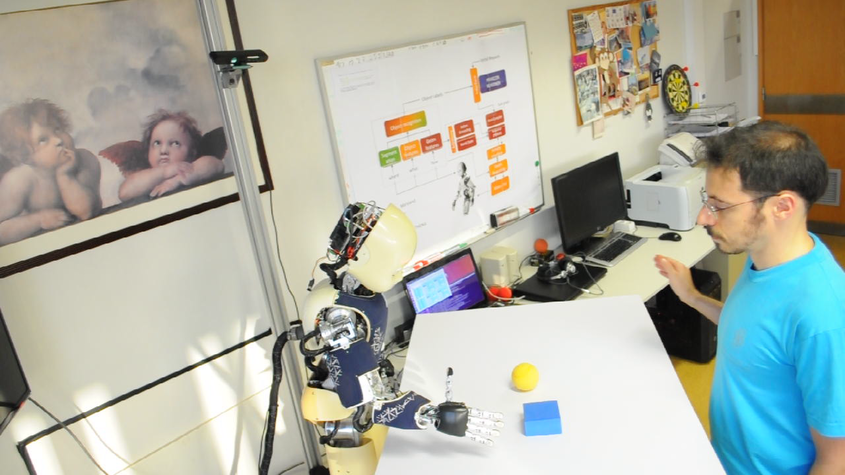
\includegraphics[width=\myWidth\linewidth]{seq2-grasp-12} } \quad
%     %
%     \subfloat
%     { 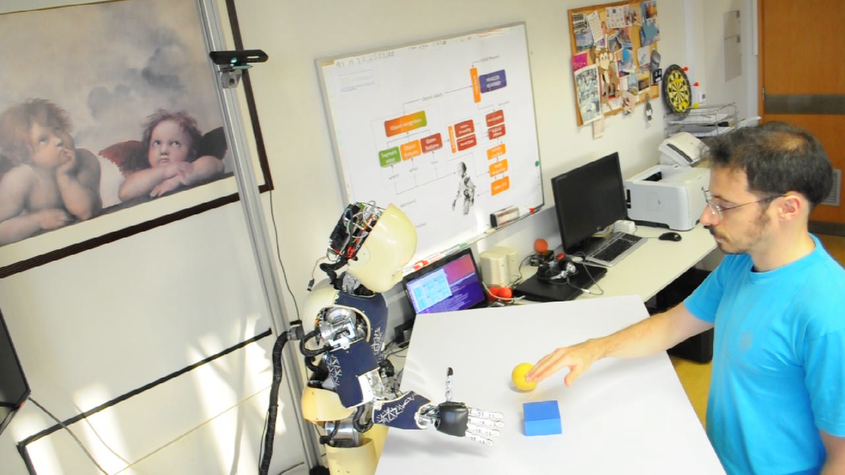
\includegraphics[width=\myWidth\linewidth]{seq2-grasp-13} } \\
%     %
%     \subfloat
%     { 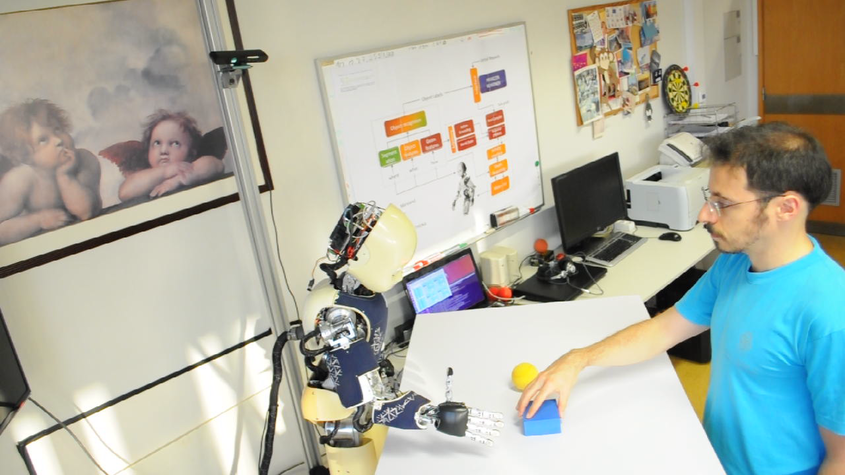
\includegraphics[width=\myWidth\linewidth]{seq2-grasp-14} } \quad
%     %
%     \subfloat
%     { 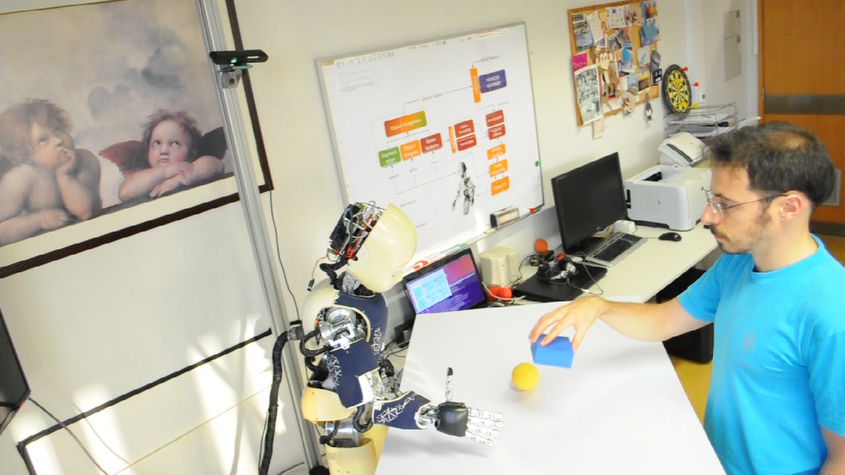
\includegraphics[width=\myWidth\linewidth]{seq2-grasp-15} } \quad
%     %
%     \subfloat
%     { 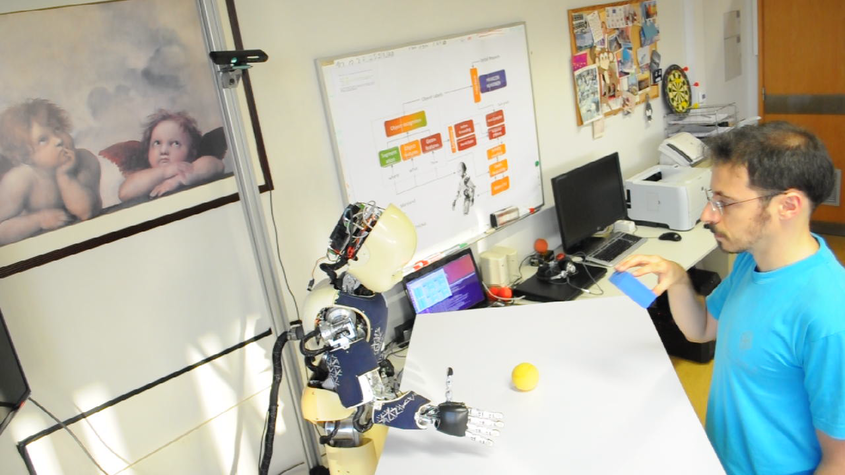
\includegraphics[width=\myWidth\linewidth]{seq2-grasp-16} }
%     \caption{grasp}
% \end{figure*}
%
% \begin{figure*}
%     \centering
%     \subfloat
%     { 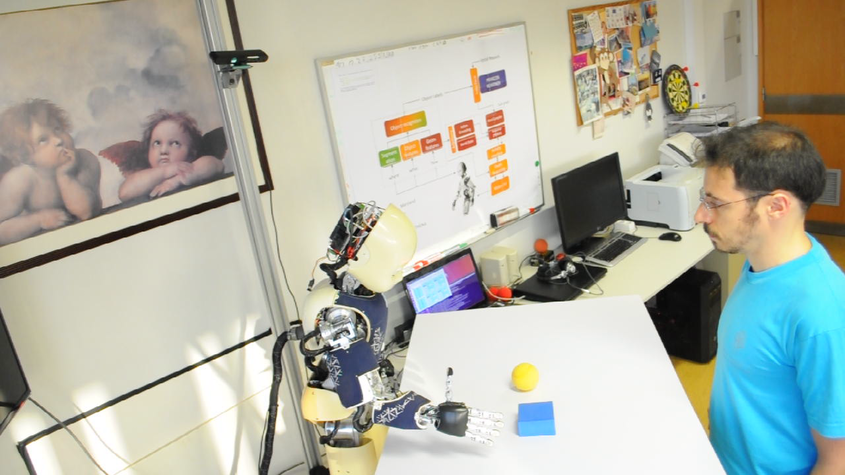
\includegraphics[width=\myWidth\linewidth]{seq2-tap-22} } \quad
%     %
%     \subfloat
%     { 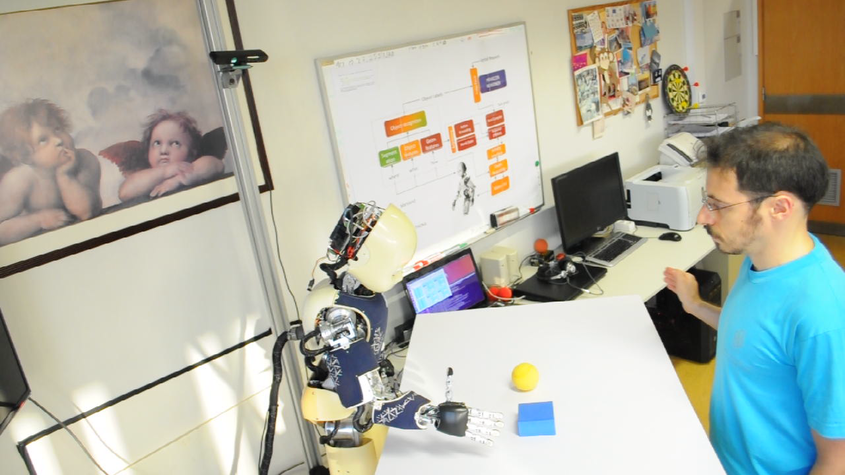
\includegraphics[width=\myWidth\linewidth]{seq2-tap-23} } \quad
%     %
%     \subfloat
%     { 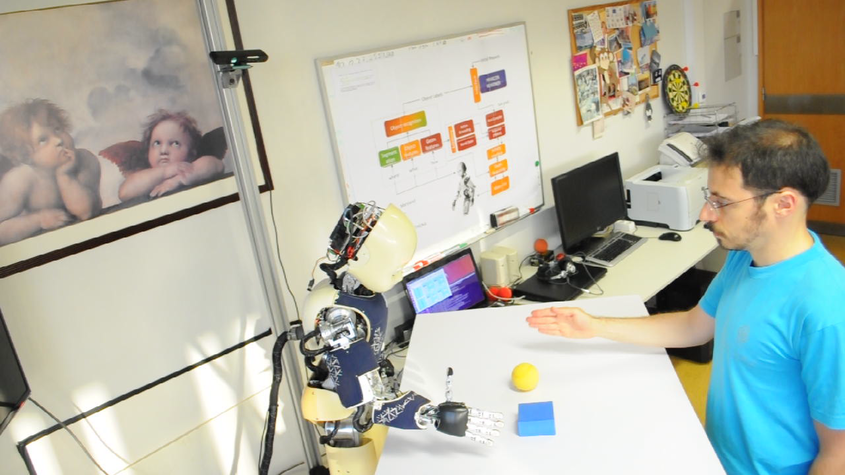
\includegraphics[width=\myWidth\linewidth]{seq2-tap-24} } \\
%     %
%     \subfloat
%     { 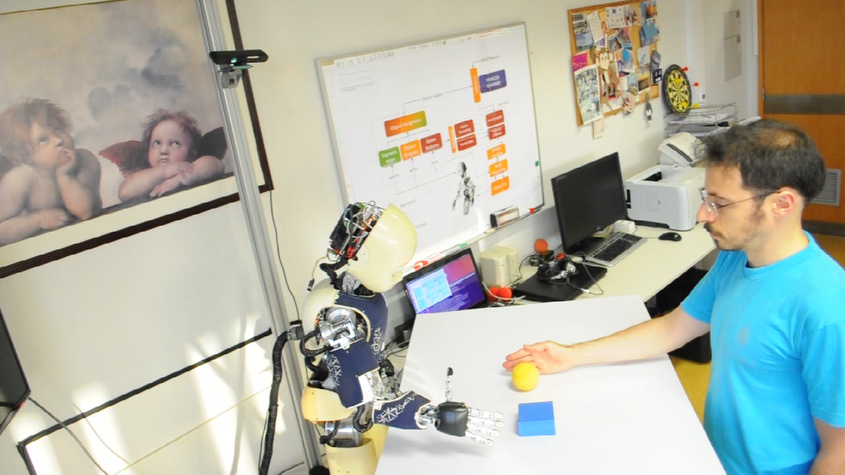
\includegraphics[width=\myWidth\linewidth]{seq2-tap-25} } \quad
%     %
%     \subfloat
%     { 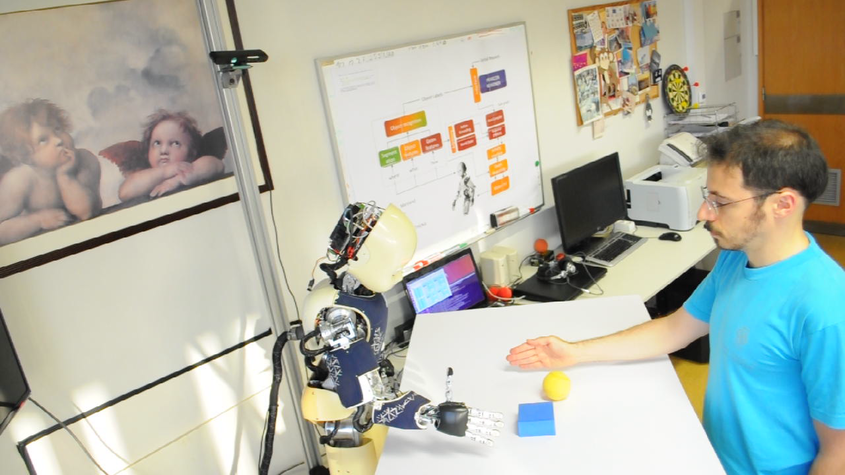
\includegraphics[width=\myWidth\linewidth]{seq2-tap-26} } \quad
%     %
%     \subfloat
%     { 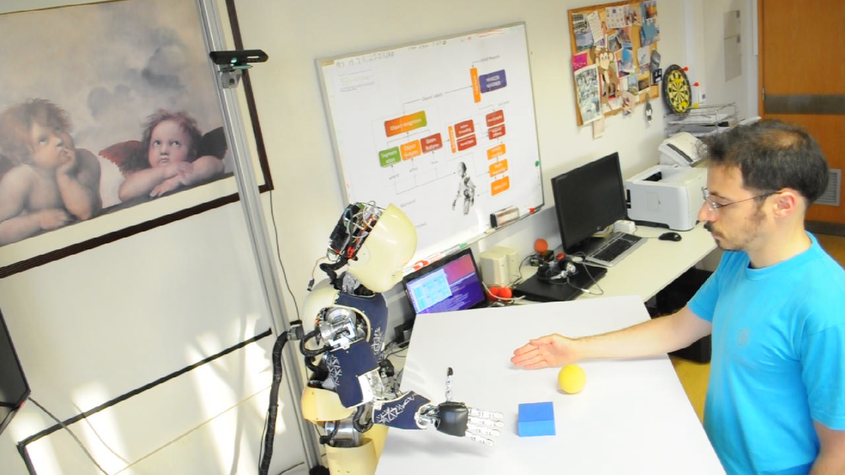
\includegraphics[width=\myWidth\linewidth]{seq2-tap-27} }
%     \caption{tap}
% \end{figure*}
%
% \begin{figure*}
%     \centering
%     \subfloat
%     { 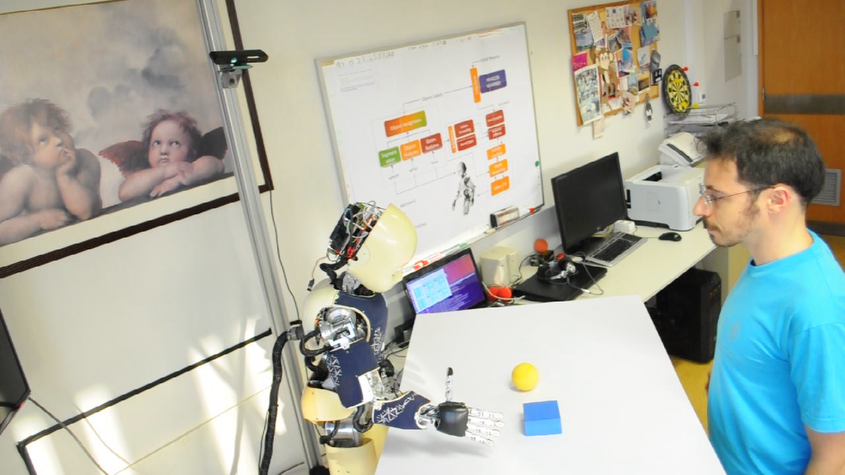
\includegraphics[width=\myWidthTwo\linewidth]{seq2-touch-2} } \quad
%     %
%     \subfloat
%     { 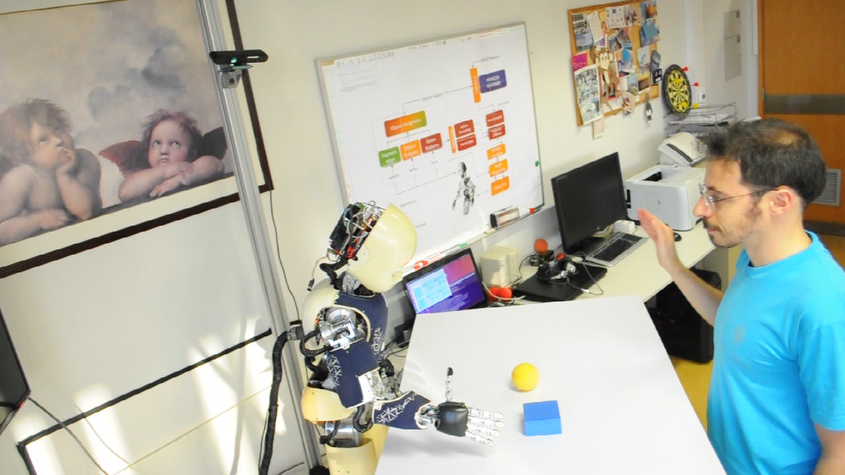
\includegraphics[width=\myWidthTwo\linewidth]{seq2-touch-3} } \quad
%     %
%     \subfloat
%     { 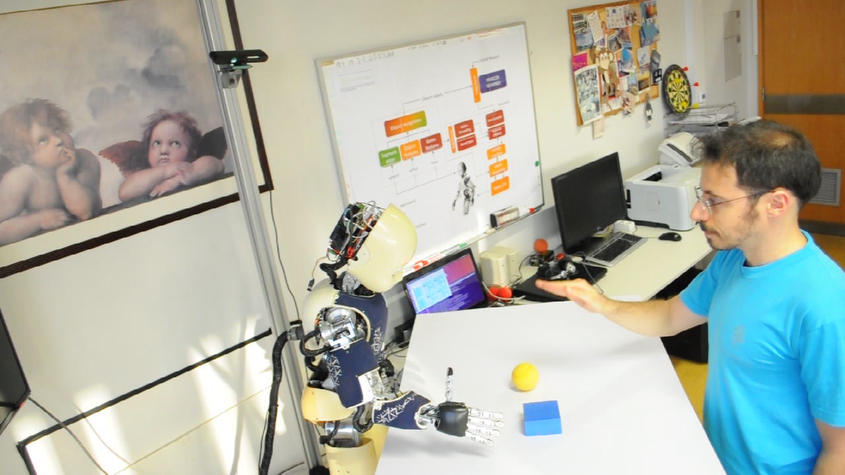
\includegraphics[width=\myWidthTwo\linewidth]{seq2-touch-4} } \quad
%     %
%     \subfloat
%     { 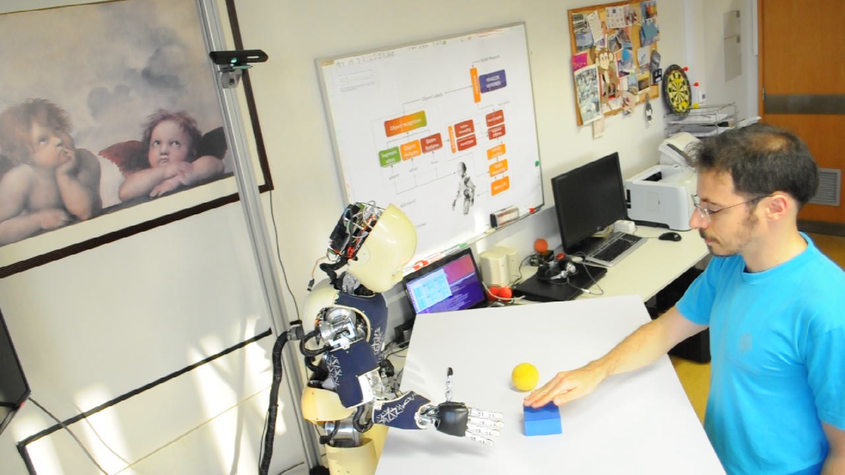
\includegraphics[width=\myWidthTwo\linewidth]{seq2-touch-5} } \\
%     %
%     \subfloat
%     { 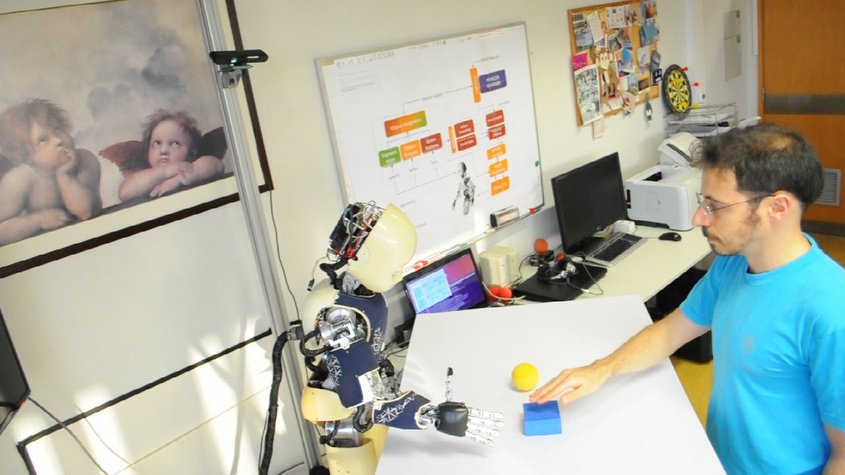
\includegraphics[width=\myWidthTwo\linewidth]{seq2-touch-6} } \quad
%     %
%     \subfloat
%     { 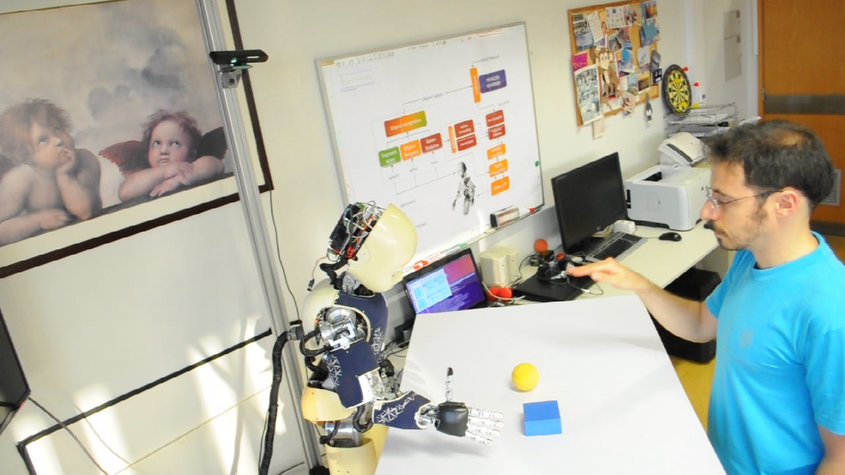
\includegraphics[width=\myWidthTwo\linewidth]{seq2-touch-7} } \quad
%     %
%     \subfloat
%     { 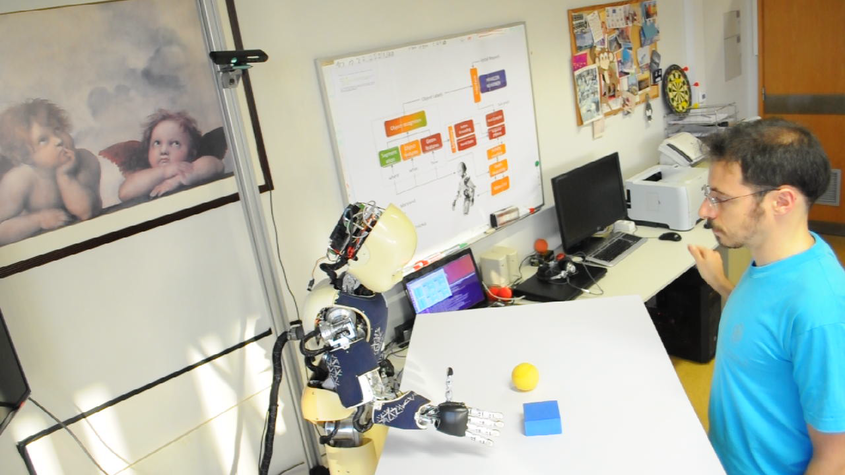
\includegraphics[width=\myWidthTwo\linewidth]{seq2-touch-8} } \quad
%     %
%     \subfloat
%     { 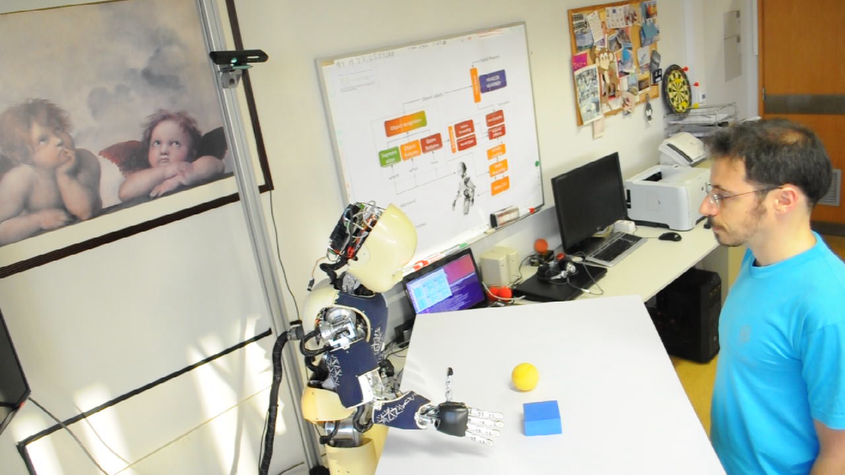
\includegraphics[width=\myWidthTwo\linewidth]{seq2-touch-9} }
%     \caption{touch}
% \end{figure*}
